\documentclass[12]{article} %the sets the document type.

\usepackage{amsmath,amssymb,amsthm} %this loads commonly used math packages
\usepackage{enumitem}
\usepackage{float}
\newtheorem{theorem}{Theorem} %this declares the theorem environment
\setlist[enumerate]{leftmargin=*,widest=0}
\usepackage{graphicx}
\graphicspath{ {boolesResources/} }
\usepackage{multicol}
\setlength{\columnsep}{1cm}

\title{George Boole}
\author{Nick Zayatz and Michele Burns}

\renewcommand{\baselinestretch}{1.5} 
\begin{document} %document starts here
\maketitle % makes the title

Over the course of his life, George Boole made some major contributions to mathematics. In the field of analysis, Boole published his treatise \textit{Applications to the Theory of Definite Integrals On the Comparison of Transcendents, with Certain Applications to the Theory of Definite Integrals} in 1857. In this work, Boole mainly studies the sum of residues of rational functions. A residue is most simply described as a complex number that is proportional to the line integral of a complex function that is complexly differentiable on its entire domain except for a few select points. These residues are calculated by functions in the form $f: \mathbb{C}\setminus \{a_{k}\}_{k} \rightarrow \mathbb{C}$, where $f$ is complexly differentiable on all points except $\{a_{k}\}_{k}$. Boole's work in this field eventually lead him to the equality which we now call Boole's Identity. This identity states that $\forall a_{k},b_{k}, \text{ and } t \in \mathbb{R}$ where $a_{k} > 0 \text{ and } t > 0$, then the following identity is true:

\begin{figure}[H]
\centerline{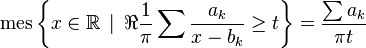
\includegraphics[scale=0.8]{boolesIdentity}.}
\caption{Boole's Identity for residues of rational functions.}\label{fig1}
\end{figure}

Boole also did some minor work in the study of probability. In the second part of his \textit{An Investigation of The Laws of Thought} (1854), Boole used his new discoveries in symbolic logic in an attempt to determine whether or not events would happen based on what passed events had previously occurred. This section of his work contains the outlines of what we know now as the \textbf{union bound} or Boole's Inequality. Boole's Inequality states that the probability of any specific event occurring in a set of events is less that the sum of the probabilities of all of the events in that set. This can be expressed in mathematical terms by the inequality

\begin{eqnarray*}
\mathbb{P}\bigg(\bigcup\limits_{i} A_{i}\bigg)\leq\sum\mathbb{P}(A_{i})
\end{eqnarray*}\\
where $A_{i}$ is representative on an event in the set. This inequality was later perfected and generalized by Carlo Emilio Bonferroni in the 1930's.

Despite his contributions to other mathematical fields, Boole's most important addition to the development of mathematics was his work involving symbolic logic, which many now refer to as "Boolean Algebra." Boole first introduced this topic of study in his treatise \textit{The Mathematical Analysis of Logic} in 1847. The idea was then further expanded and refined in 1854, when Boole published his most famous work \textit{An Investigation of The Laws of Thought.} Boolean Algebra is a base-2 branch of algebra where each variable represents either a $true$ or $false$ value (typically $1 = true \text{ and } 0 = false$). Operations can then be performed on these values to, in essence, solve whether or not some expression will be true. Some examples of these operations are defined in Figure \ref{fig2}. 

\begin{figure}[H]
\centerline{Negation: if $x$ is $true$, then the expression (Not $x$) is $false$}
\centerline{And: if the values $x$ and $y$ are both $true$, then the expression ($x$ and $y$) is $true$}
\centerline{Or: if either $x$ or $y$ is $true$, then the expression ($x$ or $y$) is $true$}
\caption{Definitions for some Boolean Algebra operations.}\label{fig2}
\end{figure}

In \textit{An Investigation of The Laws of Thought}, Boole first laid out the notation and axioms of his symbolic logic. Each operation has numerous forms, the most common of which can be seen in Figure \ref{fig3}.

\begin{figure}[H]
\centerline{Variables: $x,y,z$}
\centerline{Negation: $(1-x), -x, \bar{x}, !x$}
\centerline{Or: $x\cup y, x$ or $y, x + y, x | y$}
\centerline{And: $x \cap y, x$ and $y, xy, x*y, x \& y$}
\centerline{True: $1$, true, $T$}
\centerline{False: $0$, false, $F$}
\caption{Various forms of notation for Boolean Algebra operations.}\label{fig3}
\end{figure}
\noindent
The axioms of Boolean Algebra can be seen in Figure \ref{fig4}.

\begin{figure}[H]
\begin{equation*}
\begin{aligned}[c]
&1.\text{ Identity:}		&	&2.\text{ Null Value:}		&	&3.\text{Complement:}\\
&x*1 = x				&	&x*0 = 0				&	&x*\bar{x} = 0\\
&x + 0 = x				&	&x + 1 = 1				&	&x + \bar{x} = 1\\
&4.\text{ Idempotent:}	&	&5.\text{ Commutative:}	&	&6.\text{ Associative:}\\
&x*x = x				&	&x*y = y*x				&	&x*(y*z) = (x*y)*z\\
&x + x = x				&	&x + y = y + x			&	&x+(y+z) = (x+y)+z\\
&7.\text{ Distributive:}	&	&8.\text{ Inverse:}		&	&9.\text{ Absorption:}\\
&x*(y+z) = x*y + y*z		&	&\bar{\bar{x}} = x		&	&x+(x*y) = x\\
&(x+y)(x+z) = x + (y*z)	&	&					&	&x*(x+y) = x
\end{aligned}
\end{equation*}
\caption{Boole's original axioms for his symbolic logic.}\label{fig4}
\end{figure}

After laying out his guidelines for symbolic logic, Boole began to explain his mathematical concepts in terms of sets. For example, say the set $x$ denoted all metal things and the set $y$ denoted all sharp things. This would imply that the set $\bar{x}$ is the set of all non-metals, and the set $(xy)$ is the set of all sharp metals. He then explained to the reader that the variables were not simply sets of entities, rather they were questions representing properties of an entity. The variable $x$ does not represent the set of all metal things, it actually portrays the question "is the given substance a metal?" If the substance is a metal, $x$ is $1$, otherwise, $x$ is $0$. 

\newpage

\begin{thebibliography}{9}
\bibitem{AnalysisBook} 
Boole, George. 
\textit{Applications to the Theory of Definite Integrals On the Comparison of Transcendents, with Certain Applications to the Theory of Definite Integrals}. 
London: Philosophical Transactions, 1857. 745-803. Print.
 
\bibitem{BooleanBook2} 
Boole, George. 
\textit{An Investigation of the Laws of Thought: On Which Are Founded Mathematical Theories of Logic and Probabilities}.
New York: Dover, 1854. Print.
 
\bibitem{MacTutor} 
"George Boole."
\textit{Boole Biography}.
JOC/EFR, June 2004. Web. 16 Feb. 2016. 
\end{thebibliography}

\end{document}